\renewcommand\TheFile{hardware.tex}
\SVN $Author: hom $
\SVN $Revision: 12 $
\SVN $Id: hardware.tex 12 2012-11-28 10:01:49Z hom $
\SVN $Date: 2012-11-28 11:01:49 +0100 (Wed, 28 Nov 2012) $
\SVN $State: Exp $
\begin{savequote}[8cm]
  \sffamily
  Those parts of the system that you can hit with a hammer (not
  advised) are called hardware; those program instructions that you
  can only curse at are called software.
  \qauthor{Anonymous}
\end{savequote}
\chapter{Control of the elevator hardware}

\section{The hardware elevator}
\parpic(40mm,30mm){
  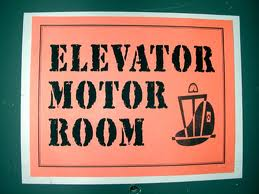
\includegraphics[width=40mm]{figures/elevatormotorroom.jpeg}}
The purpose of the software product is to control a scale
hardware model of an elevator system. The model elevator has n floors,
numbered 0 to n-1. For our current hardware model n=4.

This simple system has the following controllable elements.

\vspace{7mm}
\begin{Enumerate}
\item A cage to transport passengers.
\item Up buttons, one each for the floors 0..n-2 to request a cage to
  a floor to move up.
\item Down buttons, one each for the floors 1..n-1 to request to a
  floor to move down.
\item n target buttons, inside the cage to request the floor to stop
  at a floor to let the passenger(s) out.
\item A simulated door. In the current model the door is simulated
  with four LEDs. These LEDs are controlled with two inputs and two
  output. This simulated door is assumed to be closed when all LEDs
  are lit and (fully) open when all LEDs are off. This information is
  available via the \texttt{door closed} respectively \texttt{door open} sensor. The LEDs switch on
  from left to right and switch off from right to left to simulate a
  moving door. See figure~\ref{fig:doortiming}
  \vpageref[below]{fig:doortiming}.
\item A red button inside the cage.
\item A sensor for each floor, telling that the bottom of the cage
  meets the floor level.
 \item A bidirectional motor. The motor's purpose is to hoist and
  lower the cage.
\item Direction LEDs which show the intended direction of travel of
  the cage, visible from the floor.
\item Floor indicator LEDs to indicate where the cage is at the
  moment. When the cage is at a floor the matching indicator is
  lit. When the cage is between floors, both the indicator for the
  floors below and above the cage should be lit.
\item Open and close buttons for the elevator door, located inside the
  cage.
\item Obstruction sensor to reopen the doors when a passenger is
  between the doors.
\item A test button which can be used to simulate the nurse mode button.
\end{Enumerate}

\begin{figure}[htbp]
  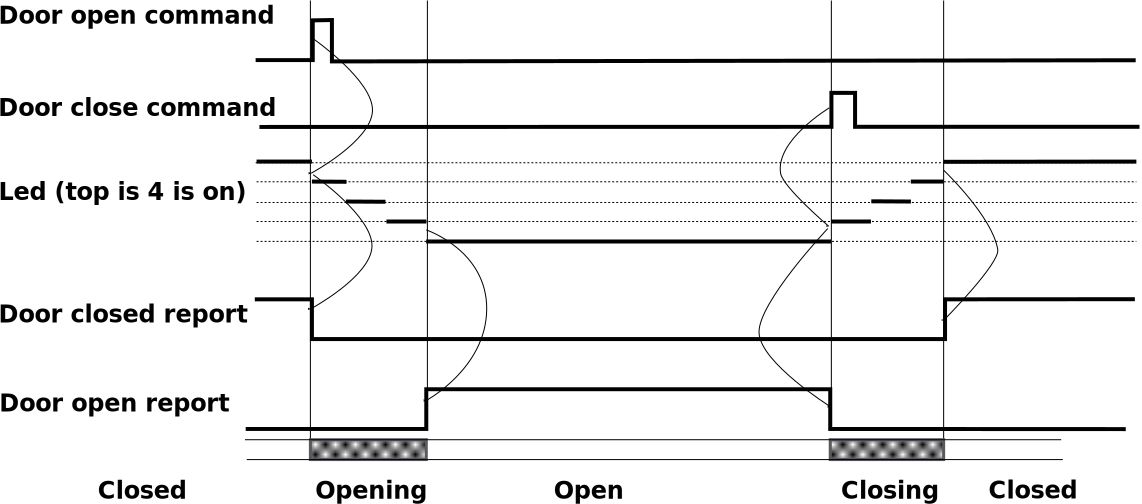
\includegraphics[width=\textwidth]{figures/doorsim}
  \caption{\label{fig:doortiming}Door timing diagram}
\end{figure}

\section{Input and outputs controlling the hardware model}

The elevator model is connected using the io-Warrior chip. This allows
control of 32 io bits. In the hardware 11 bits outputs and 21 bits are
used. The connections are listed in table~\ref{tab:connections} \vpageref[below]{tab:connections}.

\begin{table}[htbp]
  % \small
  \centering
  \caption{\label{tab:connections}Hardware connections of the elevator
    model}
  \shadowbox{
    \begin{tabular}{crcl}
      \textbf{in/out} & \textbf{bitNr} &\textbf{warrior bit}& \textbf{control} \\\hline
      in  & 0 & P0.0 & up button 0         \\
      in  & 1 & P0.1 & up button 1         \\
      in  & 2 & P0.2 & up button 2         \\
      in  & 3 & P0.3 & down button 1       \\\hline

      in  & 4 & P0.4 & down button 2       \\
      in  & 5 & P0.5 & down button 3       \\
      in  & 6 & P0.6 & door closed sensor  \\
      in  & 7 & P0.7 & red cage button (alarm button) \\\hline
      
      in  & 8 & P1.0 & target button 0     \\
      in  & 9 & P1.1 & target button 1     \\
      in  & 10 & P1.2 & target button 2     \\
      in  & 11 & P1.3 & target button 3     \\\hline

      in  & 12 & P1.4 & floor sensor 0      \\
      in  & 13 & P1.5 & floor sensor 1      \\
      in  & 14 & P1.6 & floor sensor 2      \\
      in  & 15 & P1.7 & floor sensor 3      \\\hline

      out& 16 & P2.0 & floor indicator light 0 \\
      out& 17 & P2.1 & floor indicator light 1 \\
      out& 18 & P2.2 & floor indicator light 2 \\
      out& 19 & P2.3 & floor indicator light 3 \\\hline

      out & 20 & P2.4 & Motor down bit       \\
      out & 21 & P2.5 & Motor up bit     \\
      out & 22 & P2.6 & door open cmd     \\
      out & 23 & P2.7 & buzzer (avoid)/blue led test   \\\hline\hline
\multicolumn{4}{c}{\textbf{Bits below are extensions on previous hardware}}\\\hline
      in  & 24 & P3.0 & (nurse button) (test)\\
      out & 25 & P3.1 & up led    \\
      out & 26 & P3.2 & down led   \\
      out & 27 & P3.3 & door close cmd \\\hline

      in  & 28 & P3.4 & door open sensor  \\
      in  & 29 & P3.5 & door open button \\
      in  & 30 & P3.6 & door close button \\
      in  & 31 & P3.7 & obstruction sensor \\\hline

\multicolumn{4}{p{80mm}}{\textbf{All bits are in true logic. A one
    activates LED or motor-bit, a 0 turns it off. For inputs: a 1 is
    an activated 
    sensor or button, a 0 is the inactive state.}}\\\hline
    \end{tabular}
  }
\end{table}

\begin{wrapfigure}{r}{60mm}
  \vspace{-1\baselineskip}
  \begin{center}
    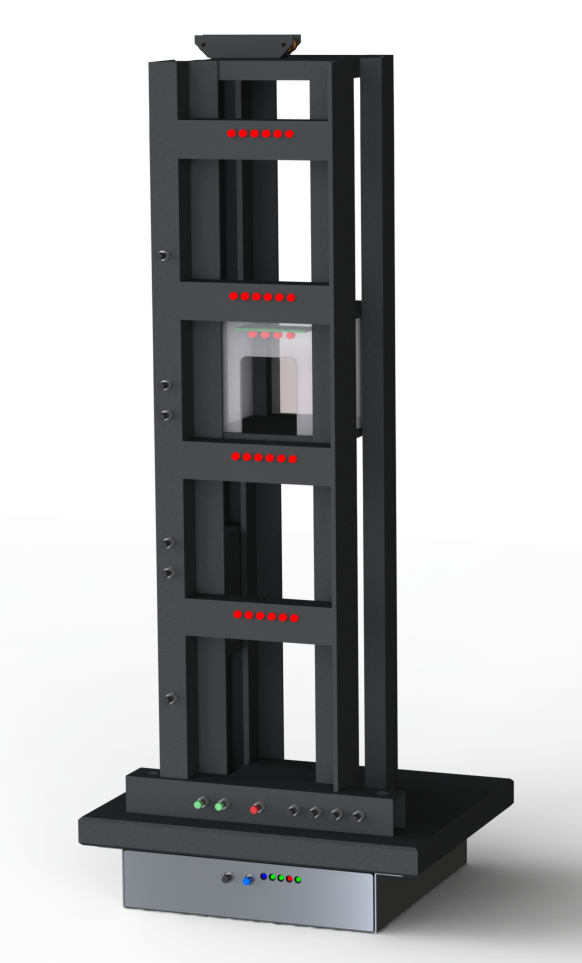
\includegraphics[width=58mm]{figures/lift2.png}
  \end{center}
  \vspace{-1\baselineskip}
  \caption{Elevator model}
  \label{fig:lift}
  \vspace{-1\baselineskip}
\end{wrapfigure}
Notes: The door LEDs are not in the output list. They are controlled
with the door open and close command bits and can be monitored with the door
opened and closed sensor as can be seen in figure~\ref{fig:doortiming}
\vpageref[above]{fig:doortiming}. 

The elevator motor is controlled with two bits. It has two LEDs
connected, one for up and one for down, which light up when the motor
is switched on in that direction. The LEDs are on the bezel or
pedestal, out of sight of the passenger.

Left and right of the floor indicator lights on
each floor, there is one up and down LED. These LEDs should show the
travel direction chosen by the elevator control. These up/down LEDs
should go off when the elevator has no more calling or moving passengers.

In this project the hardware model is connected using the IO warrior
chip. This is then connected to the USB port of a computer (PC or
MAC). 

The inputs and outputs are pure binary, which allows  the use of one
bit for each of the inputs and outputs. An active bit has value 1 in
the aggregate, an inactive bit value 0.

\section{IO operations provided  by the IO Warrior}

The operations provided by the IO Warrior development kit can be found
in the Java documentation. For your convenience we provide a copy of
the IOwarrior software development kit  api at
\url{http://prj32.fontysvenlo.org/iowarrior-SDK/Java/doc/api/index.html}. 
The SDK can also be found at the prj32 web page \url{http://prj32.fontysvenlo.org/}.

To get you started and to remove some startup and shutdown issues we
provide a few utility classes in the package \lstinline{sevenlohwio}.
This package and some more packages is also available in the
project repository.


\subsection{Bit operations}
\lstset{language=Java}
The basic read and write operations on most computer binary IO is word
wide, in which the word with is 8, 16 or 32 bits at a time.
In most smaller systems, including the PC, the minimum amount is 8
bits or a byte. In the case of the IOWarrior we have an USB Human
intarface device. We use the IOWarrior in its simplest mode, in which
case its provides access to it IO pins with read and write of all the
32 bits at a time.
As an abstraction we define two interfaces that should implemented and
on which you can design and implement a complete binary IO subsystem.

The basic operations defined in the interfaces are 
\lstinline{int read()} and \lstinline{void write(int v)}. Implementing these
interfaces enables encapsulation of the IO device in classes. The
object of such an implementation class could for instance encapsulate
an IOWarrior or a network connection to an iowarrior connected to
another computer. The identification of the proper port and connector or
IOWarrior address should be taken care of in the constructor in the
class design, which assigns the port and card info to final fields.

Specific to the IOWarrior is that it behaves as a so called Human
Interface USB device, that is, it behaves similar to a keyboard or
mouse. This implies that a read operation only returns if there is
input. Such a operation is called a \textit{blocking} operation. 

Your main task in the project related to IO is to provide bit handling.
In particular you will have to implement the detection of the
input bit changes and notification of observers or listeners.
Of course you will have to design and implement the bit output
operations as well. 

We strongly suggest that you make use of a change-Listener design,
which is similar to an instance of the \Okis{Observer Pattern}
combined with \Okis{Adapter}. The listeners are then driven by a
method, \lstinline{void pollOnce()} defined in the interface 
\textbf{Poller} that periodically or regularly interrogates the 
input word.

In the class diagram in figure~\ref{fig:listener} you find part of the
hwio library. The white classes and interfaces are the ones that you
might want to extend or implement. In particular you will want to
implement \Code{BitListener}(s) and the \Code{AbstractBitFactory},
which produces \Code{InBit} and \Code{OutBit} Objects or derivatives
of thereof.
\begin{figure}[htbp]
  \centering
  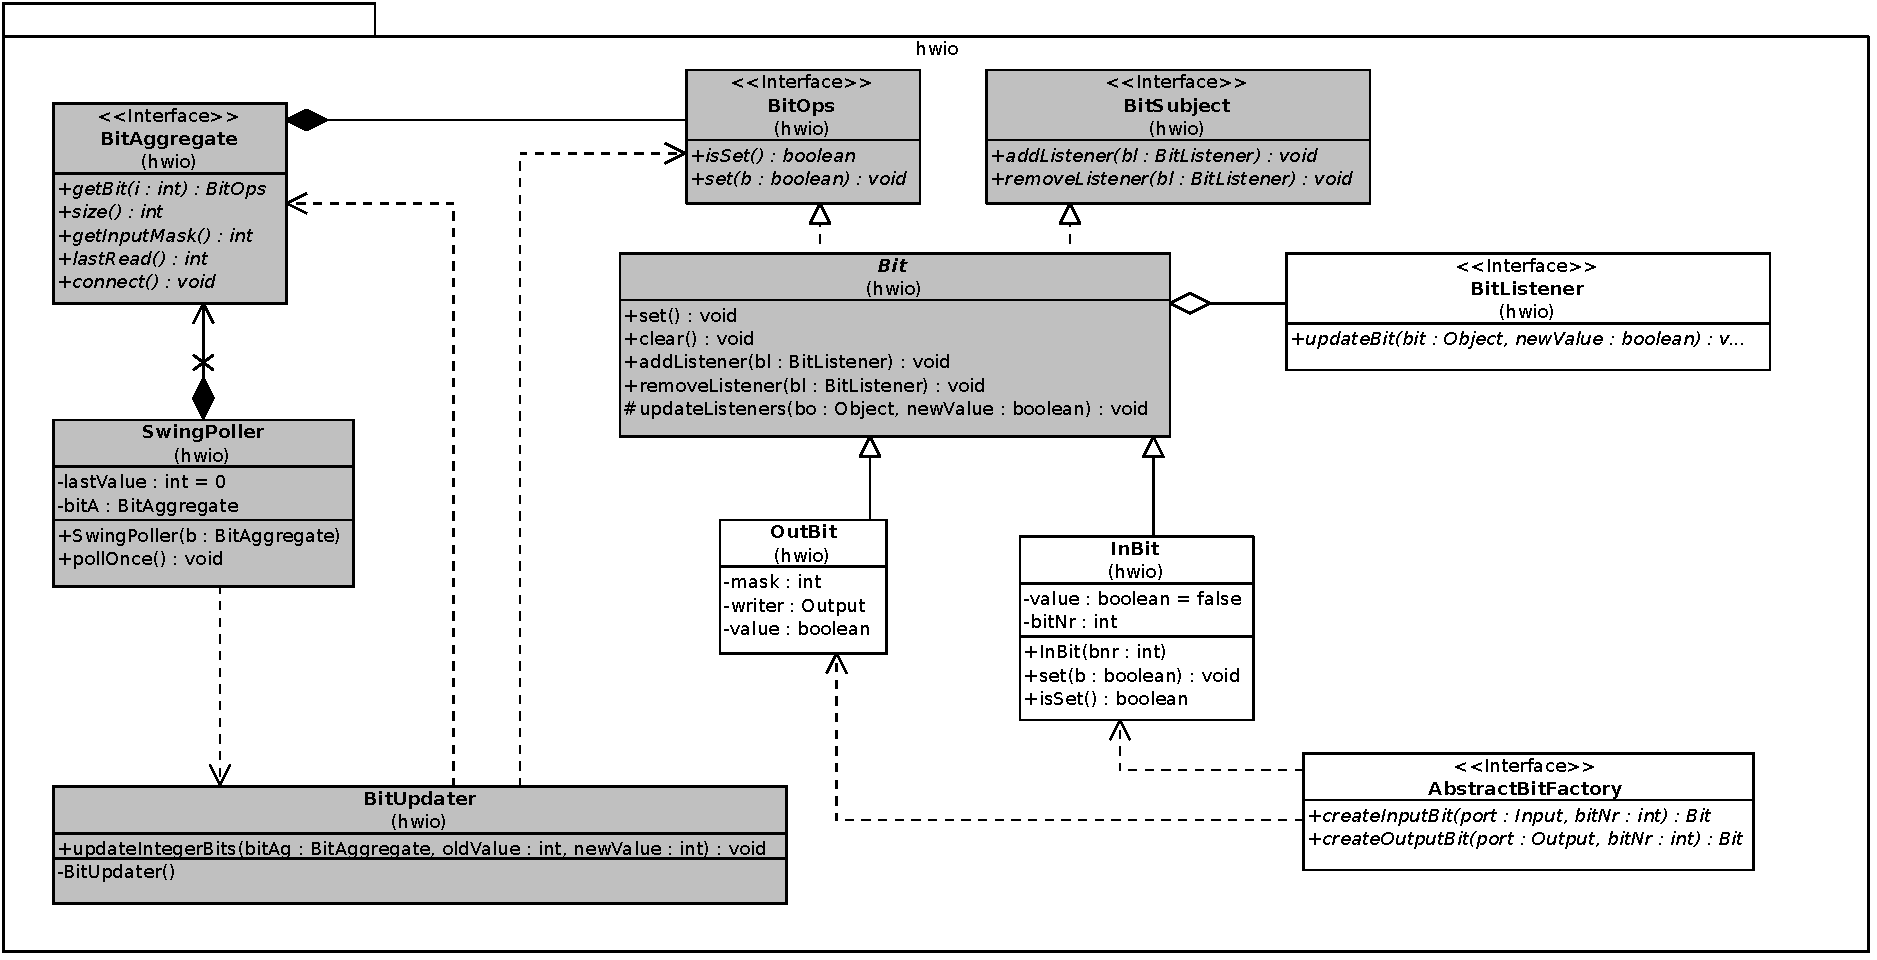
\includegraphics[width=\textwidth]{figures/hwio.pdf}
  \caption{Bit Listener class diagram of sevenlohwio}
  \label{fig:listener}
\end{figure}

\subsection{Bit handling}

To be able to isolate or operate on bits in word\footnote{Word is any
  group of bits in this context, in the examples you will see groups
  of 8, named octet or \lstinline{byte}, but \lstinline{short}, \lstinline{integer} and \lstinline{long} are also words
  in this context.} you need a few bitwise logical operation.

\begin{description}
\item[NOT] inverts all bits in a word, that is a 0
  becomes a 1 and a 1 becomes zero. Mathematical example:
  \texttt{
    \begin{eqnarray*}
      \begin{aligned}
        a      &=& 0101 & 0101\\\hline
        \lnot a &=& 1010 & 1010\\
      \end{aligned}
    \end{eqnarray*}}
  The Java (and C) symbol for the bitwise not operator is $\tilde{ }$ as
  in \lstinline{~a}.
\item[AND] a bit in the result is 1 if all the corresponding bits in
  all arguments are 1, else 0. Mathematical example:
  \texttt{
    \begin{eqnarray*}
      \begin{aligned}
        a         &=& 0100& 0101\\
        b         &=& 0001& 1111\\\hline
        a \land b &=& 0000& 0101\\
      \end{aligned}
    \end{eqnarray*}}
  The Java symbol is the single ampersand (\&) as in \lstinline{r = a & b}.
\item[OR] a bit in the result is 1 if the any of the corresponding bits in the
  arguments is one, else 0. Mathematical example
  \texttt{
    \begin{eqnarray*}
      \begin{aligned}
        a        &=& 0100& 0101\\
        b        &=& 0001& 1111\\\hline
        a \lor b &=& 0101& 1111\\
      \end{aligned}
    \end{eqnarray*}}
  The Java symbol is the single vertical bar ($|$)  as in \lstinline{r = a | b}.
  
\item[XOR] exclusive or. A bit in the result is 1 if exactly one of
  the corresponding bits is 1.
  \texttt{
    \begin{eqnarray*}
      \begin{aligned}
        a          &=& 0100& 0101\\
        b          &=& 0001& 1111\\\hline
        a \oplus b &=& 0101& 1010\\
      \end{aligned}
    \end{eqnarray*}}
  The Java symbol is the hat (\^\ )  as in \lstinline{r = a ^ b}. With two
  arguments the xor operation tells you which of the bits differ in the
  arguments.  
\end{description}

A summary of the logical operations with two one bit arguments is given
table~\ref{tab:logops}

\begin{table}[htbp]
  \caption{\label{tab:logops}Some logical operations}
  {    \renewcommand\arraystretch{1.7}
  \begin{tabular}{IccI>{\columncolor[gray]{.8}}cc>{\columncolor[gray]{.8}}cc>{\columncolor[gray]{.8}}cc>{\columncolor[gray]{.8}}cI}\whline
    \multicolumn{9}{IcI}{Logical operations (in bit wise programming notation)}\\\whline
    \multicolumn{2}{IcI}{semantics}
    & inverse & all (both) & at least one& unequal & equal & not all & none\\\whline
    \multicolumn{2}{IcI}{math sym}
      & $\neg a$ & $a\land b$         & $a\lor b$ & $a\oplus b$
      & $a=b$    & $\neg(a \land b)$ & $\neg(a \lor b)$ \\\whline
      \multicolumn{2}{IcI}{techn. not.}
      & $\overline{a}$ & $a\cdot b$ & $a+b$ & $a\oplus b$
      &$a=b$ & $\overline{a\cdot b}$ & $\overline{a+b}$\\\whline
      \multicolumn{2}{IcI}{C style. not.}
      & $\tilde{\ }a$ & $a \& b$ & $a|b$ & $a\hat{\ } b$
      &$a=\,=b$ & $\tilde{ }(a \& b)$ & $\tilde{ }(a|b)$\\\whline
    $a$ & $b$ & not(a) & and & or & xor & equals & nand & nor \\\whline 
    0 & 0 & 1      &  0  &  0 &  0  &  1     & 1    & 1   \\
    0 & 1 & 1      &  0  &  1 &  1  &  0     & 1    & 0   \\
    1 & 0 & 0      &  0  &  1 &  1  &  0     & 1    & 0   \\
    1 & 1 & 0      &  1  &  1 &  0  &  1     & 0    & 0   \\\whline
  \end{tabular}
}

\end{table}

